\chapter{Asking Millionaires What They Are Investing In}

We begin where the host begins: not with a theorem, but with a survey. The School of Hard Knocks question --- what are people actually investing in right now? --- is posed repeatedly, and that repetition is the lecture's organizing device. Each answer adds one local mechanism: defensive equity selection, compounding, discipline under drawdown, values-based spending, self-investment, patience in a rising-rate market, and finally the passage from investing to collecting. These notes preserve that sequence and are curated for this volume by LazyingArt LLC. Where the lecture gives only a verbal mechanism, we write the lightest mathematics that keeps the argument clear without pretending that the source itself is a blackboard derivation.

\section{Opening Survey}

James begins by fixing the search space. Before anyone tells us what to buy, avoid, or trust, the lecture names the principal buckets of interest: stocks, real estate, and cryptocurrency. The point of the opening is methodological. We are not yet inside a doctrine; we are defining the domain over which later judgments will range.

\begin{equation}
\mathcal{A}
=
\{\text{Cryptocurrency},\ \text{Real Estate},\ \text{Stocks/Public Markets}\}.
\end{equation}

This set is deliberately coarse. Its function is not to classify all investable things once and for all, but to tell us what the host is about to sample in the street.

\begin{figure}[htbp]
\centering

\includegraphics[width=0.86\textwidth]{lecture_139_figure_02.png}
\caption{Opening montage of crypto, real estate, and public-market investing.}
\end{figure}

The screenshot remains in the chapter because it shows the lecture's own visual framing: crypto at upper left, real estate at upper right, and public markets below. The chart fragments in the lower panel, including visible numbers such as \(3.15\%\) and \(325\), are generic market imagery rather than trustworthy lecture data, so we keep the frame for layout and emphasis, not for quantitative evidence.

\begin{figure}[htbp]
\centering
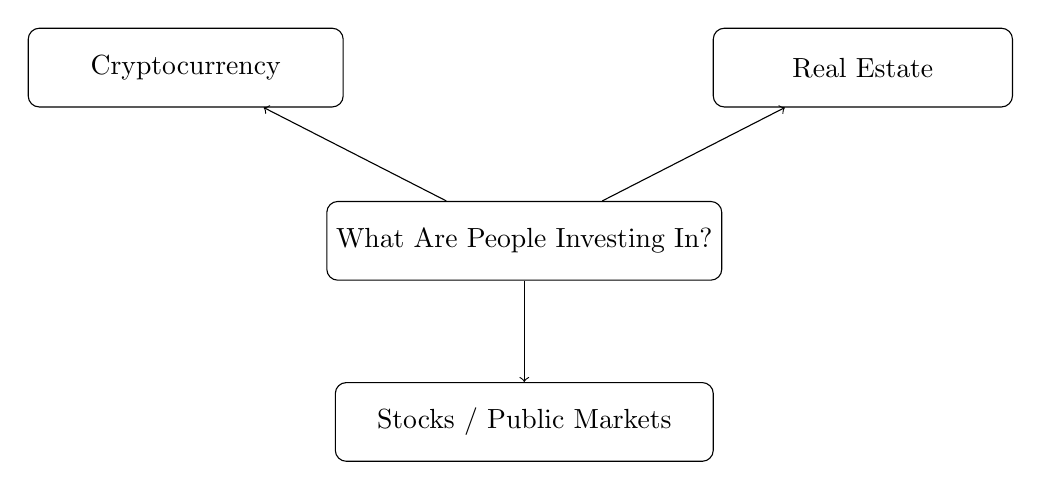
\begin{tikzpicture}
\node[draw, rounded corners, minimum width=4.2cm, minimum height=1cm] (center) at (0,0) {What Are People Investing In?};
\node[draw, rounded corners, minimum width=4.0cm, minimum height=1cm] (crypto) at (-4.3,2.2) {Cryptocurrency};
\node[draw, rounded corners, minimum width=3.8cm, minimum height=1cm] (realestate) at (4.3,2.2) {Real Estate};
\node[draw, rounded corners, minimum width=4.8cm, minimum height=1cm] (stocks) at (0,-2.3) {Stocks / Public Markets};
\draw[->] (center) -- (crypto);
\draw[->] (center) -- (realestate);
\draw[->] (center) -- (stocks);
\end{tikzpicture}
\caption{A cleaned reading of the lecture's opening asset map.}
\end{figure}

The redrawn diagram is intentionally simpler than the screenshot. It preserves the lecture's visible taxonomy without misreading the decorative stock panel as if it were a usable chart.

\section{Skepticism, Dividend Stocks, and Compounding}

The first respondent begins at a greater distance from finance than we might expect. The initial advice is epistemic rather than allocative: do not simply believe what you are told; figure things out for yourself. The reason is that there are now many forces at work --- algorithmic ones among them --- and the old implication
\[
x \longmapsto y
\]
no longer feels dependable. One could once imagine a more legible ladder: correct the visible defects, behave well enough, and the institution would gradually return money and status. The speaker even reaches for the older language of the Peter Principle, as if to mark a world in which institutional promotion once had a more recognizable shape.

From that diagnosis, the lecture pivots into portfolio behavior. If the environment is harder to read, one response is not maximal aggression but a more defensive consistency. The speaker's answer is conservative high-dividend stocks.

\paragraph{Claim.}
These stocks do not participate as strongly in euphoric markets, but they also do not absorb the full damage of bad ones.

\paragraph{Mechanism.}
A cautious way to encode that asymmetry is
\begin{align}
R_{\text{good}}^{\text{div}} &< R_{\text{good}}^{\text{mkt}}, \\
\left|R_{\text{bad}}^{\text{div}}\right| &< \left|R_{\text{bad}}^{\text{mkt}}\right|.
\end{align}
This is not a measured estimate from the lecture. It is the compact mathematical form of the verbal claim: muted upside in the boom, smaller drawdown in the slump.

\subsection{Question \& Answer}

The lecture now asks its first genuinely technical question: how can someone become financially free in 2022? The answer is pointedly anti-magical. Compounding is your friend, and therefore one year is usually too short a horizon.

Let \(W_n\) denote wealth after \(n\) periods, let \(r\) denote the effective periodic return, and let \(C_{n+1}\) denote the next contribution. Then the natural update rule is
\begin{equation}
W_{n+1} = (1+r)W_n + C_{n+1}.
\end{equation}

This is the right place for the mathematics because the lecture itself is moving from slogan to mechanism. Once we say ``compounding,'' we should write the update explicitly. Iterating the recursion gives
\begin{equation}
W_n = W_0(1+r)^n + \sum_{k=1}^{n} C_k(1+r)^{\,n-k}.
\end{equation}

The derivation is simple and worth keeping visible:
\begin{enumerate}
\item Start with \(W_{n+1} = (1+r)W_n + C_{n+1}\).
\item Replace \(W_n\) by \((1+r)W_{n-1} + C_n\).
\item Continue this substitution until the initial wealth \(W_0\) appears.
\item Collect the factors of \((1+r)\) multiplying the older contributions.
\end{enumerate}

For constant contributions \(C_k=C\), the familiar special case is
\begin{equation}
W_n = W_0(1+r)^n + C\,\frac{(1+r)^n-1}{r}.
\end{equation}

\begin{figure}[htbp]
\centering
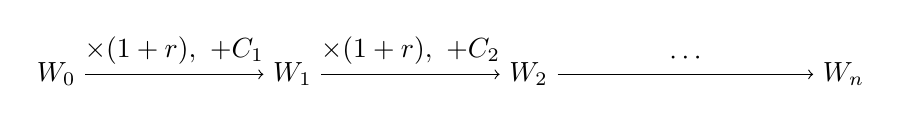
\begin{tikzpicture}
\node (w0) at (0,0) {$W_0$};
\node (w1) at (3,0) {$W_1$};
\node (w2) at (6,0) {$W_2$};
\node (wn) at (10,0) {$W_n$};
\draw[->] (w0) -- node[above] {$\times(1+r),\ +C_1$} (w1);
\draw[->] (w1) -- node[above] {$\times(1+r),\ +C_2$} (w2);
\draw[->] (w2) -- node[above] {$\cdots$} (wn);
\end{tikzpicture}
\caption{A discrete compounding picture: growth and fresh contributions arrive together.}
\end{figure}

We can now see why the speaker rejects the fantasy of one-year financial freedom. Unless the initial capital, the contribution stream, or the return rate is extraordinary, the mechanism needs time. The lecture's first serious answer is therefore not ``find the perfect asset,'' but ``choose a rule that becomes stronger as time passes.''

\section{Energy, Drawdowns, and Character}

The next interview changes the emotional temperature. A retired military man, now in consulting, says he is invested in energy stocks and is presently hunkered down because the market has fallen sharply that day. The lecture shifts at once from asset class to stress condition.

We may summarize the day's shock as
\begin{equation}
\Delta I_{\text{day}} < -1000\ \text{points},
\end{equation}
where \(\Delta I_{\text{day}}\) is only a stress marker. The transcript gives the magnitude of the fall but not a fully identified index, so the notation should remain modest.

What matters here is not that the lecture suddenly turns quantitative. It does not. Instead, it pivots from holdings to personal structure. The advice to someone leaving college is the triad
\begin{itemize}
\item intelligence,
\item integrity,
\item initiative,
\end{itemize}
followed almost immediately by another military lesson: discipline, and more precisely self-discipline.

The sequence is worth preserving exactly because it is not a trading model. The lecture wants us to see that portfolio posture and personal posture belong to the same argument. Under drawdown, the central question becomes: what kind of person can remain coherent in front of volatility? In this stretch, character is being treated as part of financial method.

\section{Human Sales and Values-Based Freedom}

The next respondent works in media and advertising, specifically in sales at TikTok. The investment answer is light and contemporary: a small dabble in crypto, then the basics in mutual funds, plus a few companies. But once again the lecture uses the allocation answer only as an entry point. The deeper move is into how one navigates economic life.

When asked about the secret to sales in 2022, the speaker answers: being human. The point is simple and concrete. The person on the other side of the transaction goes home to somebody, may have children, may need to pick someone up, may have a life that continues after the meeting ends. The lecture thus turns from instruments to relation.

\paragraph{Anecdote.}
A modest portfolio answer opens onto an account of sales that refuses to strip away the human context.

\paragraph{Claim.}
Economic success improves when we remember that the counterparty is not a revenue object but a life with constraints, habits, and obligations.

\paragraph{Mechanism.}
That same turn from abstraction to lived structure reappears in the answer to financial freedom.

\subsection{Question \& Answer}

How can someone become financially free in 2022? Here the answer is no longer compounding first. It is values-based spending. One need not begin with a wealth manager, a checklist, or an inherited financial script. One begins by identifying what one truly values and then letting the budget reflect it.

Let \(E_i\) denote spending on priority \(i\), and define the spending share
\begin{equation}
s_i = \frac{E_i}{\sum_j E_j},
\qquad
\sum_i s_i = 1.
\end{equation}
This is the minimum formalization of the idea. Freedom now depends not only on the size of the budget but on the alignment between actual expenditure shares and declared priorities.

The speaker names the priorities concretely: gym, healthy eating, organic food, travel, and other individual preferences. So the real contrast is not
\[
\text{cheap} \quad \text{versus} \quad \text{expensive},
\]
but
\[
\text{aligned} \quad \text{versus} \quad \text{unexamined}.
\]

This is the lecture's second answer to the same question, and it should remain distinct from the first. In the first answer, time is the decisive mechanism. In the second, selection is. The lecture does not ask us to choose one and discard the other; it asks us to notice that both belong to the architecture of freedom.

\section{Vocation, Degrees, and the Day-Two Reset}

At this point the lecture slows itself down. Another respondent says he should have taken youth more seriously, but the answer does not collapse into regret. Instead it opens into a music story: DJ work, then a path through CBS Records, Sony Music, and Capitol. The lecture is careful here. Seriousness is not being set against vocation; it is being asked to discipline vocation.

Then the host performs an explicit reset. This is day two. The earlier outing was thin. They came back because they wanted a broader mix: old, young, male, female, any source of a sharper sample. The chapter must keep this moment because it tells us that the lecture knows what it is doing. The repeated street question is not filler; it is the method by which the field of answers is widened.

The next cluster of responses therefore arrives under renewed motivation. A surgeon says he works in medicine, rejects college degrees in provocative language, and when asked what he is investing in names three objects in sequence:
\begin{itemize}
\item real estate,
\item himself,
\item other people he trusts.
\end{itemize}
This is a crucial widening of the investment concept. The lecture is no longer speaking only about formal assets. It is also speaking about self-capital and trusted human capital.

The same respondent's advice to his younger self is starkly compressed: no limitations. Soon after, another respondent reopens the degree question in a less absolute way, invoking examples that point in opposite directions and concluding that the real problem is inward: one has to work out one's own path. The business advice that follows has the same structure. Follow what you love closely enough that you can ask the simplest hard question: how do I monetize it?

What the lecture is doing here is easy to flatten and therefore important to preserve. It is not abandoning finance for biography. It is showing that educational choice, vocation, self-investment, and business creation all enter the wealth problem before the portfolio is fully specified.

\section{Volatility, Waiting, and the Collection Phase}

Only after this widening does the lecture return to a more explicit contrast between asset classes. The real-estate developer begins with a distinction between stocks and cryptocurrencies and then sharpens it through an analogy. Crypto is compared to a young kid: roughly \(10\) to \(15\) years old, full of energy, moving quickly. Stocks, by contrast, have been around for roughly a century.

\begin{equation}
T_{\text{crypto}} \approx 10\text{--}15\ \text{years},
\qquad
T_{\text{stocks}} \approx 100\ \text{years}.
\end{equation}

This is not a theorem about volatility; it is a disciplined analogy. The lecture uses age as a proxy for maturity and maturity as a proxy for relative stability. The conclusion is qualitative rather than econometric, but it is not empty. It tells us how the respondent wants us to feel the difference between the two objects.

\subsection{Question \& Answer}

What do we do in a tricky market? Here the lecture becomes unusually crisp. Interest rates are rising, the real-estate environment is unstable, and therefore the best trade may be not to trade. In the present market state, waiting can dominate immediate action:
\begin{equation}
V_{\text{wait}} > V_{\text{buy-now}}.
\end{equation}

\begin{figure}[htbp]
\centering
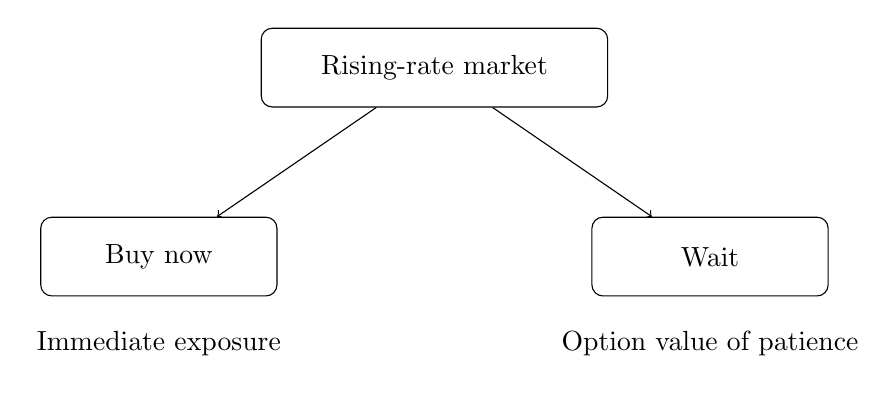
\begin{tikzpicture}
\node[draw, rounded corners, minimum width=4.4cm, minimum height=1cm] (state) at (0,0) {Rising-rate market};
\node[draw, rounded corners, minimum width=3.0cm, minimum height=1cm] (buy) at (-3.5,-2.4) {Buy now};
\node[draw, rounded corners, minimum width=3.0cm, minimum height=1cm] (wait) at (3.5,-2.4) {Wait};
\draw[->] (state) -- (buy);
\draw[->] (state) -- (wait);
\node at (-3.5,-3.5) {Immediate exposure};
\node at (3.5,-3.5) {Option value of patience};
\end{tikzpicture}
\caption{The lecture's qualitative timing split in a difficult real-estate market.}
\end{figure}

The point is not that waiting is always superior. The point is that in a rising-rate market the lecture treats non-action as a real decision, not as indecision.

The final respondent then moves the whole chapter one stage later in life. He has retired from dentistry, says that healthcare has become corporate, and gives a different kind of portfolio answer: he is done investing and now collecting. Asked what he invested in through the years, he names equities, annuities, bonds, and the things that pay every year for the rest of one's life.

That phase shift can be written as
\begin{equation}
CF_{\text{year}} = CF_{\text{eq}} + CF_{\text{ann}} + CF_{\text{bond}}.
\end{equation}
The equation is elementary by design. It marks a change of objective. We are no longer primarily accumulating optionality; we are summing annual income streams.

The lecture also preserves the practical messiness around that transition. Many financial advisors were unhelpful; one eventually was receptive; therefore the task includes continued search for competent guidance. And when the question of financial freedom appears once again, the late answer folds back toward the method of the whole video: it will take more than a year, and one part of the path is exactly what the host is doing now --- networking, asking people, learning in public. The closing advice to the young is likewise concrete: do not spend every summer in school; go try different jobs so that by the time college ends, work has already begun to separate itself into possibilities.

\section{Summary}

The lecture begins by naming an asset map and ends by enlarging it. What started as a street question about stocks, real estate, and crypto turns, step by step, into a broader inquiry about compounding, defensive positioning, character under drawdown, values-based spending, self-investment, timing, and yearly cash flow.

Its strongest pedagogical feature is that it refuses to compress these answers into a single slogan. Financial freedom is explained more than once, and each explanation arrives through a different mechanism. That is why the lecture must be written as a sequence rather than as a summary. We are meant to feel the argument unfolding: first classify the objects, then test the scripts, then write the update rule, then ask what kind of person can live through volatility, then ask what spending reveals, then ask when not to act, and finally ask what it means to stop investing and begin collecting.